\chapter{Materiais e Softwares}
% ---

% ---
\section{Microcontroladores e Microprocessadores}
% ---

Para uma melhor eficiência no processamento de dados, na década de 70
começaram a ser utilizados microprocessadores em computadores \cite{martins2005sistemas}. Os microprocessadores são componentes dedicados ao processamento de informações com
capacidade de cálculos matemáticos e endereçamento de memória externa \cite{chase2007sistemas}.

Já os microcontroladores são pequenos sistemas computacionais bastante poderosos que englobam em um único chip: interfaces de entrada/saída digitais e analógicas, periféricos importantes como a memória RAM, memória FLASH, interfaces de comunicação serial, conversores analógicos/digitais e temporizadores/contadores. Com o advento dos microcontroladores de 16 e 32 bits (atualmente o padrão é de 8bits) a capacidade de gerenciar soluções mais complexas e maior velocidade de processamento se iguala ao do microprocessador. \cite{chase2007sistemas}.

\begin{figure}[htbp]
	\centering
	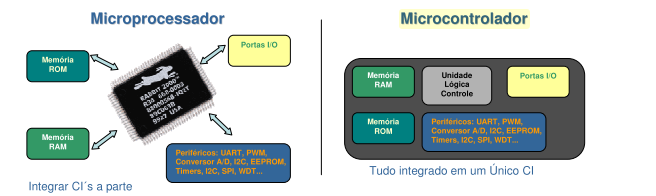
\includegraphics[scale=0.7]{figuras/processa-controla.png}
	\caption{Diferença entre microprocessador de microcontrolador}
	\label{microprocessador-microcontrolador}
\end{figure}

\subsection{ESP8266}

O ESP8266 é um circuito totalmente integrado, com interfaces de I/O digitais e analógicas e, ainda, interface WiFi, com um processador de 32 bits, capaz de executar a 160 MHz.

Os módulos baseados no microcontrolador ESP8266 representam um grande avanço na relação de preço-recursos e pode ser um componente muito interessante para soluções IoT.\cite {de2017internet}

\begin{figure}[htbp]
		\centering
		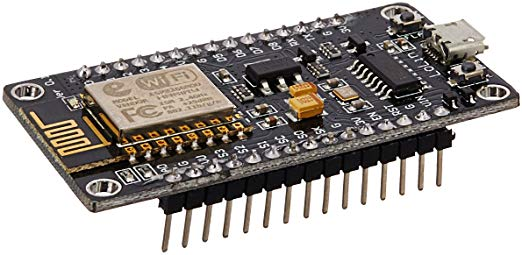
\includegraphics[scale=0.5]{figuras/esp8266_.jpg}
		\caption{ESP8266}
		\label{fig:01}
\end{figure}


\subsection{RaspberryPi}

Raspberry Pi é um minicomputador criado pela Raspberry Pi Foundation com o objetivo de estimular o ensino da ciência da computação nas escolas e universidades. Apesar de o Raspberry Pi possuir o hardware em uma única placa eletrônica de tamanho reduzido, seu potencial de processamento é significativo. O Raspberry Pi pode ser usado em diversos projetos tecnológicos, como experimentos remotos nos quais sua função é ser um Micro servidor web.\cite{crotti2013raspberrypi}

\begin{figure}[htbp]
		\centering
		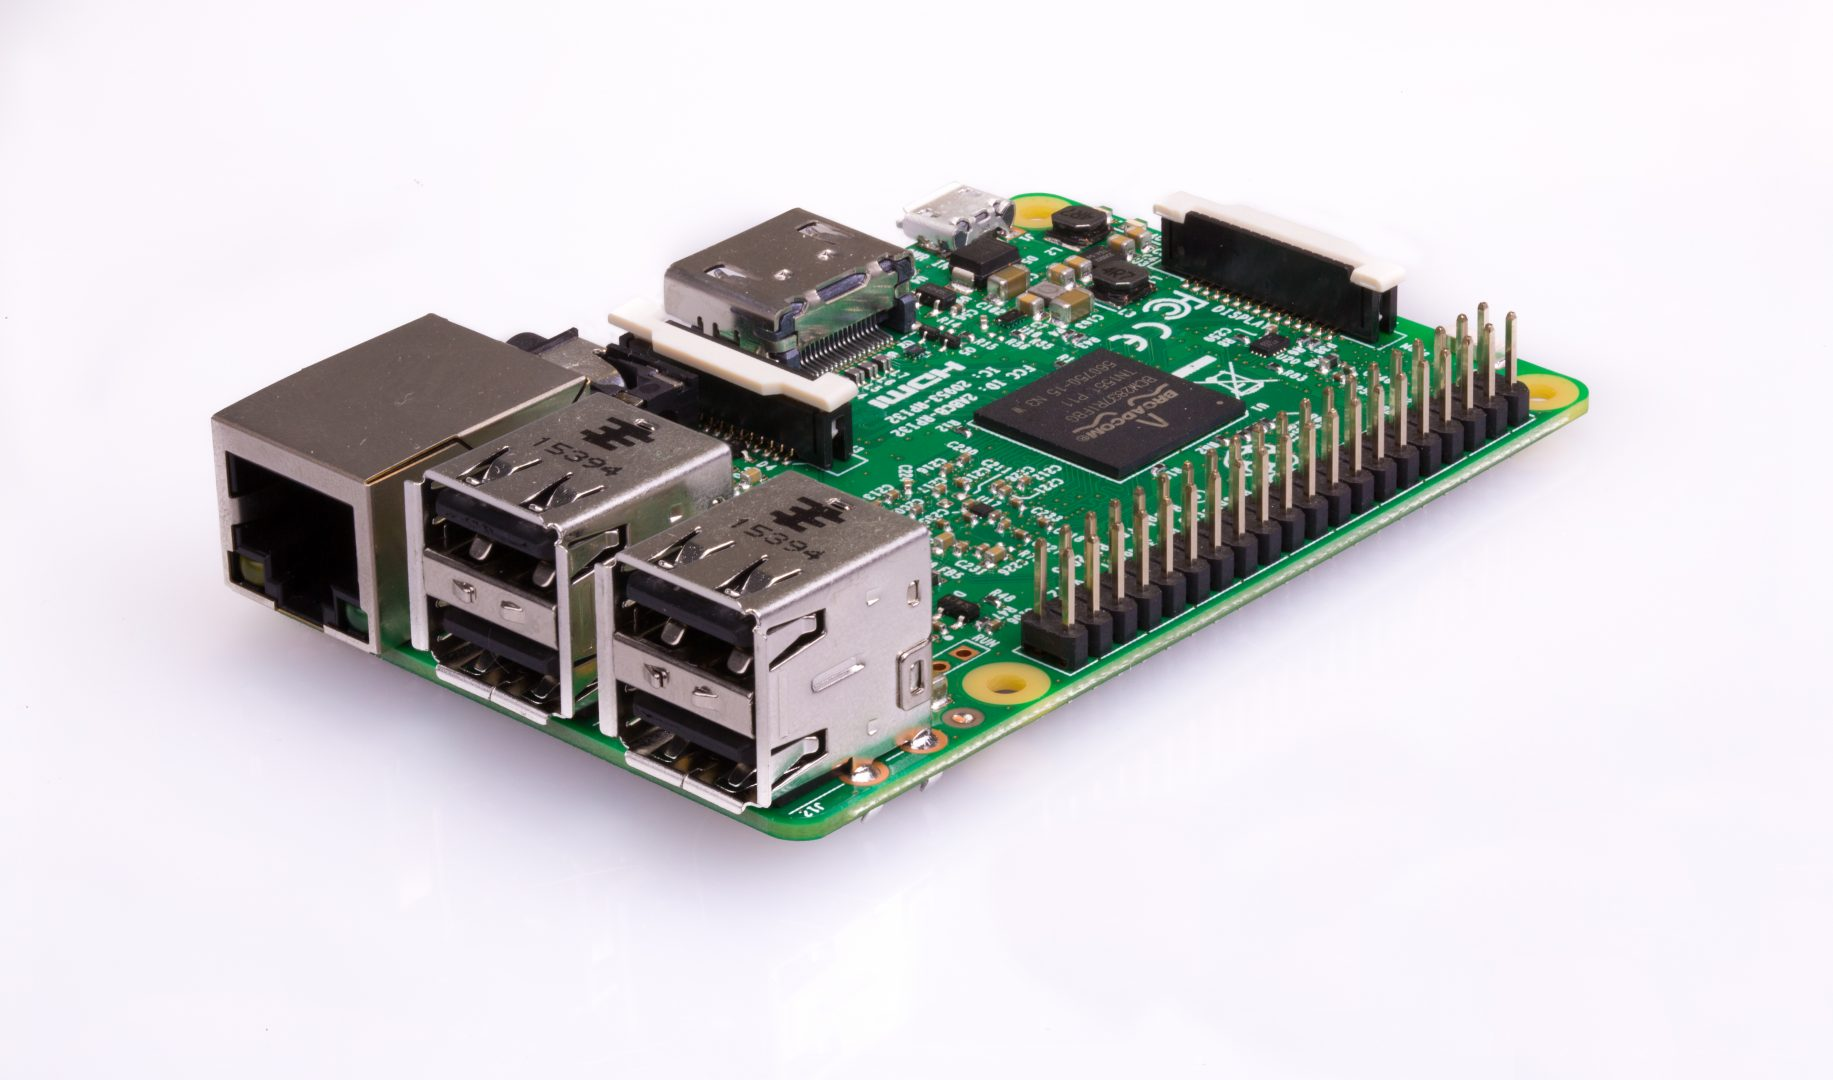
\includegraphics[scale=0.2]{figuras/raspberrypi.jpg}
		\caption{RaspberryPi}
		\label{fig:02}
\end{figure}

\section{Sensores e atuadores}

\subsection{Sensor de fluxo YF-S201}

São sensores do tipo turbina que medem a quantidade de líquido que passa pela tubulação, girando uma turbina que
gera pulsos de onda quadrada através de um sensor de efeito Hall\cite{roque2018sistema} O
sensor usa esse efeito para enviar um sinal PWM,e através desse pulso é possível mensurar a quantidade de água que passa pelo cata-vento no interior do sensor, cada pulso mede aproximadamente 2,25 mm.\cite{ms2017automaccao}

\begin{figure}[htbp]
		\centering
		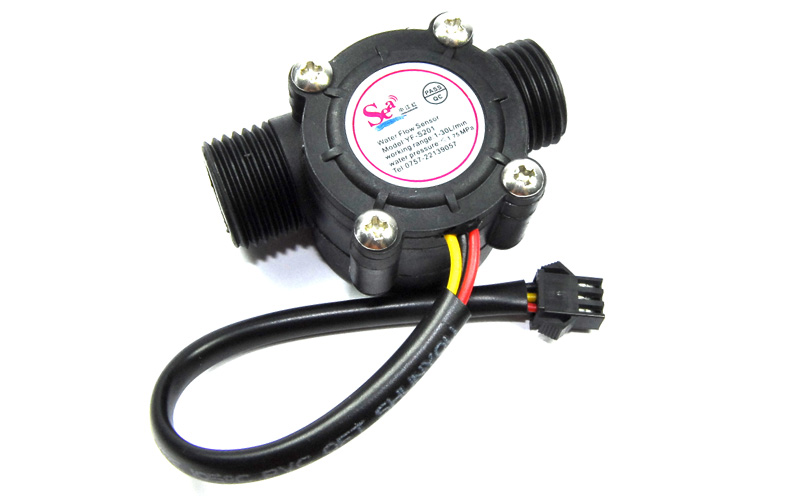
\includegraphics[scale=0.3]{figuras/yf-s201.jpg}
		\caption{Sensor de fluxo de água YF-S201}
		\label{fig:03}
\end{figure}

\subsection{Teclado matricial de membrana}

Como \cite {teclado-matricial-1} definiu, teclados são geralmente utilizados em aplicações na qual o usuário precisar interagir com um sistema, como computadores, calculadoras, controles remotos entre outros. Segundo \cite{teclado-matricial} O Teclado Matricial de Membrana 4X4 com 16 teclas foi desenvolvido com a finalidade de facilitar a entrada de dados em projetos com plataformas microcontroladas. Este teclado possui 16 teclas, onde 10 teclas são numerais, 4 literais e 2 de caracteres. As 16 teclas estão dispostas em 4 linhas por 4 colunas e o teclado possui um conector de 8 pinos para ligação.

\begin{figure}[htbp]
	\centering
	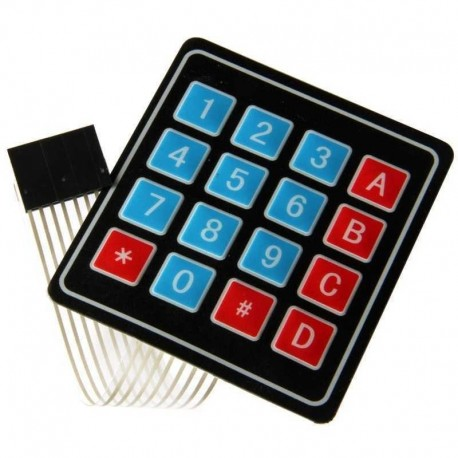
\includegraphics[scale=0.3]{figuras/teclado-matricial.jpg}
	\caption{Teclado Matricial de Membrana}
	\label{teclado}
\end{figure}

Este teclado como o nome indica é formado de botões organizados em linhas e colunas de modo a formar uma matriz. Quando pressionado, um botão conecta a linha com a coluna na qual está ligado. 

\begin{figure}[htbp]
	\centering
	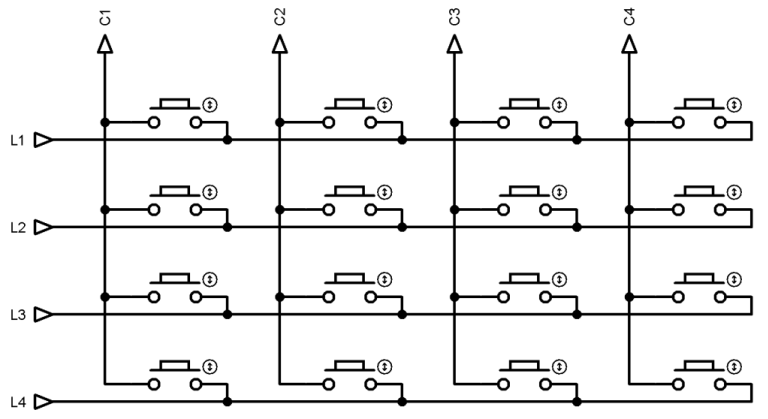
\includegraphics[scale=0.4]{figuras/matrix-1024x558.png}
	\caption{Circuito do teclado}
	\label{teclado-conexoes}
\end{figure}

O teclado matricial possui a seguinte pinagem:

\begin{itemize}
	\item Pino 1 (Esquerda) – Primeira Linha (L1)
	\item Pino 2  – Segunda Linha (L2)
	\item ...
	\item Pino 5 – Primeira Coluna (C1)
	\item ...
	\item Pino 8 – Quarta Coluna (C4)
\end{itemize}

\begin{figure}[htbp]
	\centering
	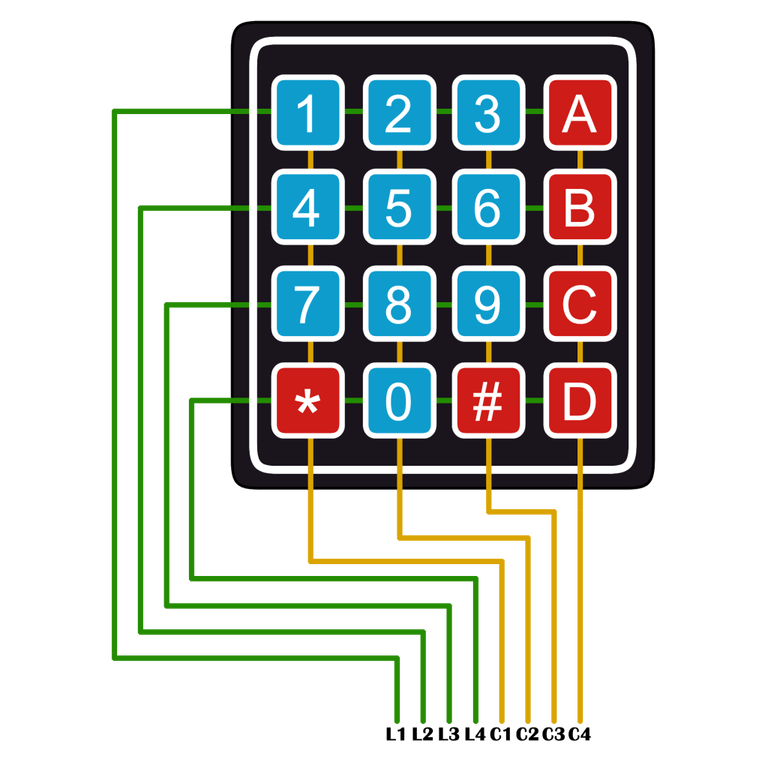
\includegraphics[scale=0.3]{figuras/keypad-1024x1024-pins.png}
	\caption{Pinagem do teclado}
	\label{teclado-pins}
\end{figure}

\subsection{Válvula solenoide}

Seguindo a definição de \cite{da2002modulo}, solenóides são dispositivos eletromecânicos baseados no deslocamento causado pela ação de um campo magnético gerado por uma bobina e são muito utilizados na construção de outros dispositivos, como é o caso das válvulas para controle de fluidos. Em particular, as válvulas para baixas vazões (da ordem de mililitros por minutos) e baixas pressões têm sido amplamente aplicadas em equipamentos e montagens para uso em laboratórios clínicos e químicos. Elas são de pequenas dimensões e requerem baixa tensão e corrente de acionamento.

\begin{figure}[htbp]
	\centering
	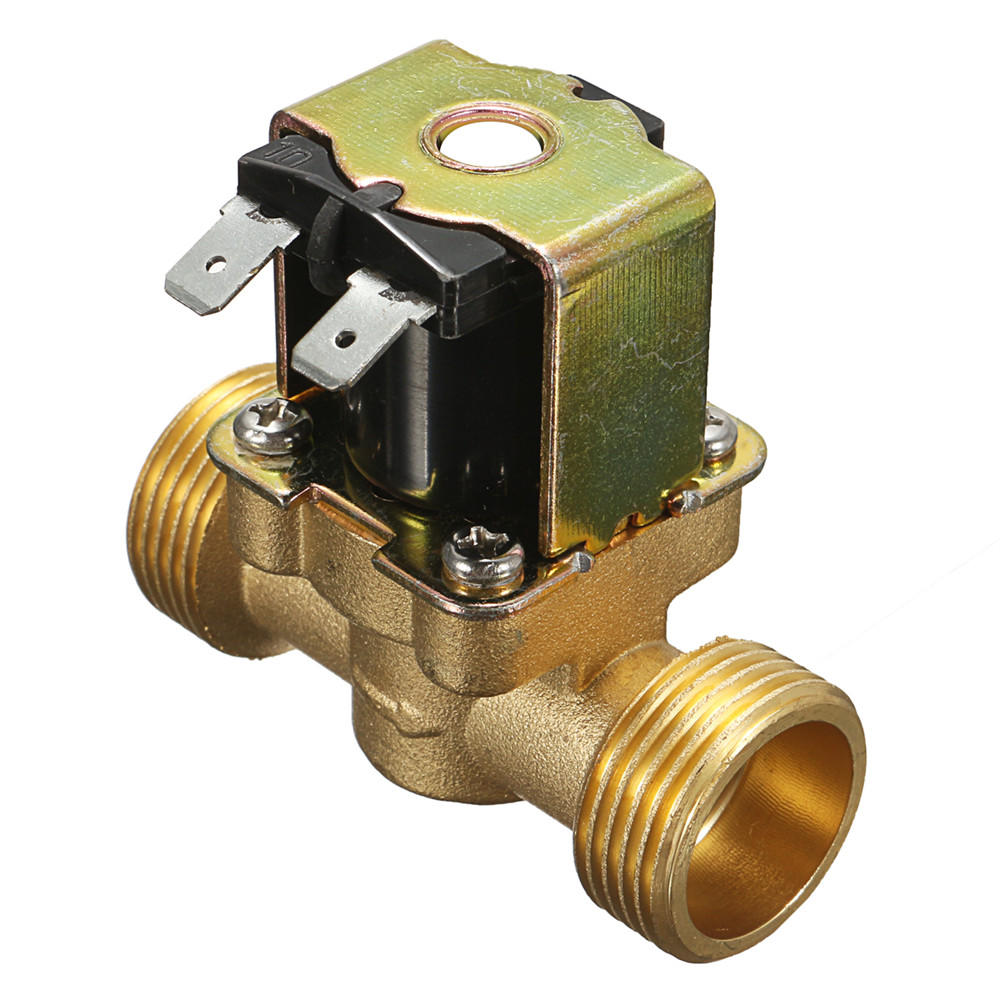
\includegraphics[width=0.3\linewidth]{figuras/valvula-solenoide.jpg}
	\caption{Válvula Solenoide}
	\label{valvula-solenoide}
\end{figure}

Ainda segundo \cite{da2002modulo}, a estratégia para fechamento e abertura dos canais fluídicos depende do fabricante, mas o princípio de acionamento elétrico é basicamente o mesmo, isto é, uma tensão de alguns volts é aplicada sobre um solenoide que faz com que um núcleo metálico ferromagnético se desloque, causando a alteração do estado da válvula. O núcleo
ferromagnético comprime uma mola que é a responsável por deslocar o núcleo para sua posição original quando a corrente elétrica é interrompida.

\section{Softwares}

\subsection{HomeAssistant}

HomeAssistant é um plataforma de automação escrita em Python. E, como \cite{Lundrigan2017} define, inclui componentes contribuídos por usuários que permite a interface com dispositivos e Web Services. Em seu núcleo, HomeAssistant é um protocolo de mensageiria, facilitando a comunicação entre dispositivo e componentes funcionais na rede provendo simples abstrações de componentes de automação residencial como sensores, câmeras, players de música, etc.

\begin{figure}[htbp]
	\centering
	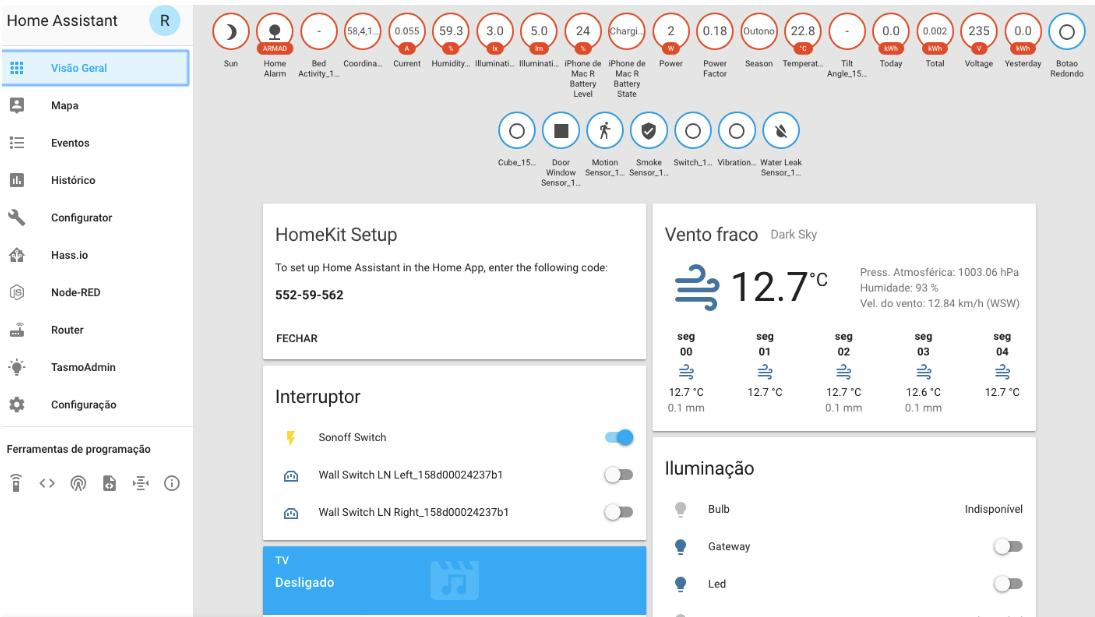
\includegraphics[width=1\linewidth]{figuras/homeassistant-dash.png}
	\caption{Dashboard genérico do HomeAssistant}
	\label{fig:homeassistant-dash}
\end{figure}

Seguindo a definição de \cite{Gomes2018}, o HomeAssistant tem suporte para diversos tipos de protocolos wireless, como BLE, ZigBee, Z-Wave e WiFi. Conta também com um RESTful API e suporta HTTP, MQTT, TCP sockets e componentes customizados. Estes componentes customizados permitem usuários a adicionar funções próprias ao HomeAssistant sem a necessidade de mudar o seu código 'core'. Isto torna a integração de novos dispositivos e sensores muito mais fácil com o Home Assistant.


HomeAssistant conta com uma grande comunidade de desenvolvedores com mais de 1.450 contribuidores e 23.700 estrelas no GitHub \cite{githubhomeassistant}, o que significa uma abundância em sua documentação sobre os seus componentes, fóruns e chats para conseguir ajuda de outros usuários, e diversos posts em blogs e vídeos sobre como começar a utilizar o programa.

Embora o Home Assistant tenha suporte à uma grande gama de protocolos wireless, este trabalho foca em sensores WiFi pois, ainda segundo \cite{Lundrigan2017}:

\begin{itemize}
	\item Hardware WiFi são mais baratos e palpáveis.
	\item WiFi é muito mais comum do que outros protocolos wireless.
	\item Sensores WiFi conseguem integrar com o resto da casa pois utiliza IP, tornando o sensor mais fácil de debugar e monitorar.
\end{itemize}

\cite{AlmeidaCosta} nos diz que o HomeAssistant instala-se em qualquer sistema operacional, suportado no Python 3 e é muito pequeno e leve, o que é excelente se quiser usar um Rasberry Pi como um hub de automação pequeno e barato. É importante lembrar que o Home Assistant age apenas como uma central de controlo que pode informar outros serviços, como o Philips Hue ou o Nest, para realizr alguma função. O Home Assistant é fácil de usar e configurá-lo é barato.

\subsection{Banco de dados de séries temporais}

Como \cite{Noor2017} define, um Banco de Dados de Séries Temporais (TSDB) é um tipo de banco que é otimizado para dados que contém traços de tempo ou séries temporais. É construído especificamente para lidar com métricas, eventos ou medidas que contém o tempo como variável. Um TSDB é otimizado para medidas que mudam com o tempo, permite o usuário criar, enumerar, alterar, destruir e organizar várias séries temporais de um método mais eficiente. A principal diferença entre bancos de séries temporais dos outros bancos de dados é que os dados que são recuperados dele são sobre o tempo. Atualmente, a maioria das empresas estão gerando uma quantidade gigante de dados sobre métricas e eventos que levam em consideração o tempo, mostrando que a necessidade de bancos de dados de séries temporais é inevitável.

Ainda segundo \cite{Noor2017}, aplicações comuns para os TSDBs são IoT, DevOps, Analise de Dados, etc. Alguns casos de uso incluem monitoramento de sistemas de software como máquinas virtuais, monitoramento de sistemas físicos como algum equipamento, dispositivos conectados, o ambiente, sistemas de automação residencial, corpo humano, etc.

\subsubsection{InfluxBD}

InfluxDB é o Banco de Dados de Séries Temporais usado neste projeto. Segundo \cite{Lundrigan2017}, InfluxDB é projetado especificamente para dados do tipo séries temporais. O que combina perfeitamente com os dados coletados do sensor que será guardado no banco.

É um projeto open-source com o opcional de armazenamento em nuvem desenvolvido por InfluxData. É escrito na linguagem de programação Go e otimizado para lidar com dados de séries temporais. Provém um linguagem de consulta parecida com o SQL. \cite{Noor2017}

\subsection{Banco de dados relacional}

Segundo \cite{bancosrelacionais}, um Banco de dados relacional possui uma coleção de tabelas, todas com nomes únicos, que compõem a base de
dados, podendo estar relacionada a uma ou mais tabelas. Conceitos como integridade referencial de dados – que garantem que um dado referenciado em uma tabela esteja presente na tabela que está sendo referenciada – e chaves primárias estão presentes e garantem que um conjunto de informações possa ser representado de maneira consistente, independente da forma de acesso.

\subsubsection{PostgreSQL}

Segundo \cite{stones2006beginning} PostgreSQL é uma excelente implementação de um banco de dados relacional, cheio de funções, de código aberto e sem custos para o uso.
PostgreSQL pode ser usado com a maioria das linguagens de programação existentes.

O PostgreSQL ganhou diversos prêmios, incluindo o \textit{Linux Journal Editor's Choice Award for Best Database} três vezes e o \textit{2004 Linux New Media Award for Best Database System}.

\subsection{Node.JS}

Node.JS, também chamado de Node, é um ambiente de servidor que utiliza a linguagem de programação JavaScript. Como \cite{Tilkov2010} define, é baseado no runtime do Google, o chamado motor V8. O V8 e o Node são basicamente implementados em C e C++, focando na performance e baixo consumo de memória. Embora o V8 suporte principalmente o uso de JavaScript no navegador, o Node foca no suporte de processos de servidores.

Segundo \cite{Sapes2016}, Node.JS utiliza um paradigma baseado em eventos e não-bloqueador de I/O, o que o torna leve e eficiente. É perfeito para aplicações de tempo real que lidam com dados intensos em dispositivos de baixo poder de processamento.

O Node é um dos ambientes e frameworks mais famosos que suportam o desenvolvimento de servidores utilizando o JavaScript. A comunidade criou um grande ecossistema de bibliotecas e vasta documentação que dão suporte ao Node. \cite{Tilkov2010}

\subsubsection{Arquitetura de microsserviços}

Seguindo a definição de \cite{ms1}, a arquitetura de microsserviços é uma abordagem no desenvolvimento de uma aplicação que baseia na existência de diversos pequenos serviços independentes. Cada um dos serviços deve rodar em seu próprio processo independente. Estes serviços podem comunicar entre si utilizando mecanismos leves de comunicação (geralmente em torno no HTTP). Os serviços devem ser absolutamente independentes.

\begin{figure}[htbp]
	\centering
	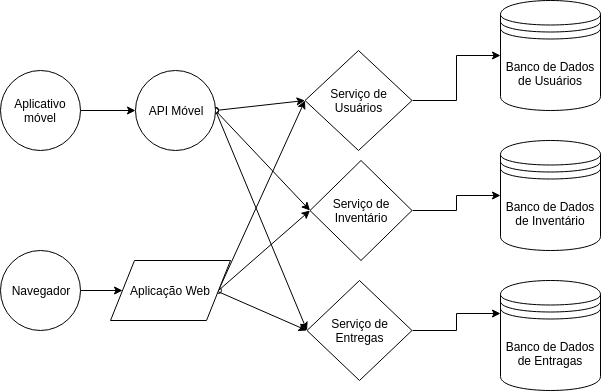
\includegraphics[width=1\linewidth]{figuras/Microservice_Architecture.png}
	\caption{Exemplo arquitetura de microsserviços}
	\label{fig:arquitetura-microsservicos}
\end{figure}

Baseado em \cite{Pahl}, microsserviços é os resultados da decomposição funcional de uma aplicação. São caracterizados pela definição de sua interface e função no sistema. Como cada serviço deve ser independente, uma alteração na sua implementação não deve afetar o funcionamento de outro serviço.

\subsection{Protocolo de comunicação}

\subsubsection{MQTT}

MQTT significa Message Queuing Telemetry Transport, é um protocolo de transporte leve que utiliza eficientemente a largura da banda de rede.\cite{mqtt1} O MQTT trabalha no TCP e garante a entrega de mensagens de um nó para um servidor. Sendo um protocolo orientado por troca de mensagens, MQTT é ideal para nós IoT, que tem recursos e capacidades limitados.

É um protocolo inicialmente desenvolvido pela IBM \cite{mqtt-ibm} em 1999, e recentemente foi reconhecido como padrão pela OASIS (Organizarion for the Advancement of Structured Information Standards).\cite{mqtt-oasis}

\cite{Kodali2017} definiou o MQTT como um protocolo baseado em \textit {publish/subscribe}. Qualquer conexão MQTT envolve dois tipos de agentes, os clientes MQTT e um MQTT \textit {broker} público, ou servidor MQTT. Os dados que são transportados pelo MQTT são referenciados como mensagens da aplicação. Qualquer dispositivo ou programa que é conectado pela rede e troca mensagens através do MQTT é chamado de cliente MQTT. Um cliente MQTT pode ser tanto um \textit {publisher} ou um \textit {subscriber}. Um \textit {publisher} publica mensagens e um \textit {subscriber} requisita a aplicação para receber mensagens. Um MQTT \textit {server} é um dispositivo ou programa que interconecta os clientes MQTT. Ele aceita e transmite as mensagens através de múltiplos clientes conectados à ele.

\begin{figure}[htbp]
	\centering
	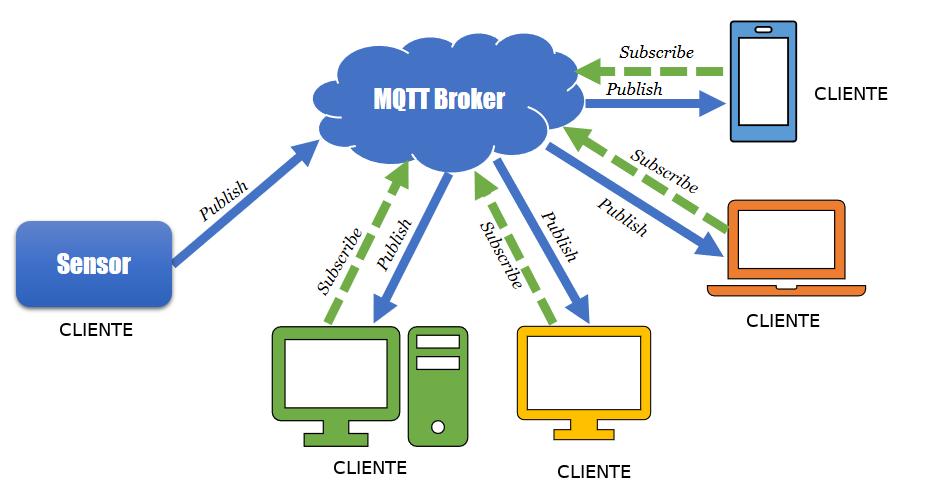
\includegraphics[width=1\linewidth]{figuras/mqtt-architecture.png}
	\caption{Exemplo da arquitetura do MQTT}
	\label{fig:arquitetura-mqtt}
\end{figure}

Dispositivos como sensores, celulares, etc. são considerados como clientes MQTT, quando um cliente MQTT tem alguma informação para transmitir, ele publica o dado para o \textit {broker} MQTT.

O \textit {broker} MQTT, ou servidor MQTT é responsável por coletar e organizar os dados. As mensagens publicadas por clientes MQTT é transmitida para outros clientes MQTT que se inscreverem ao tópico. O MQTT é desenhado para simplificar a implementação no cliente por concentrar todas as complexidades no \textit {broker}. Os \textit {publishers} e \textit {subscribers} são isolados, o que significa que eles não precisam conhecer a existência do outro.

\subsection{MQTT Mosquitto}

O Mosquitto é um \textit{broker} MQTT de código aberto \cite{Kodali2017} que entrega uma implementação padrão de servidor e cliente MQTT. Utiliza o modelo \textit{publish/subscribe}, tem uma baixa utilização de rede e pode ser implementado em dispositivos de baixo custo como microcontroladores que podem ser usados em sensores remotos de IoT. \cite{Light}

Segundo \cite{Light}, Mosquitto é recomendado para o uso sempre em que se necessita de mensagens leves, particularmente em dispositivos com recursos limitados.

O Projeto Mosquitto é um membro da Eclipse Foundation. Existem três partes no projeto:

\begin{itemize}
	\item O servidor principal Mosquitto.
	\item Os clientes mosquitto \textit{pub} e mosquitto \textit{sub}, que contém ferramentas para se comunicar com o servidor MQTT.
	\item Uma biblioteca cliente MQTT, escrita em C.
\end{itemize}